Here is a Gantt chart showing the timeline for my MMath independent project:


\begin{figure}[h] % 'h' means place it here
    \centering
    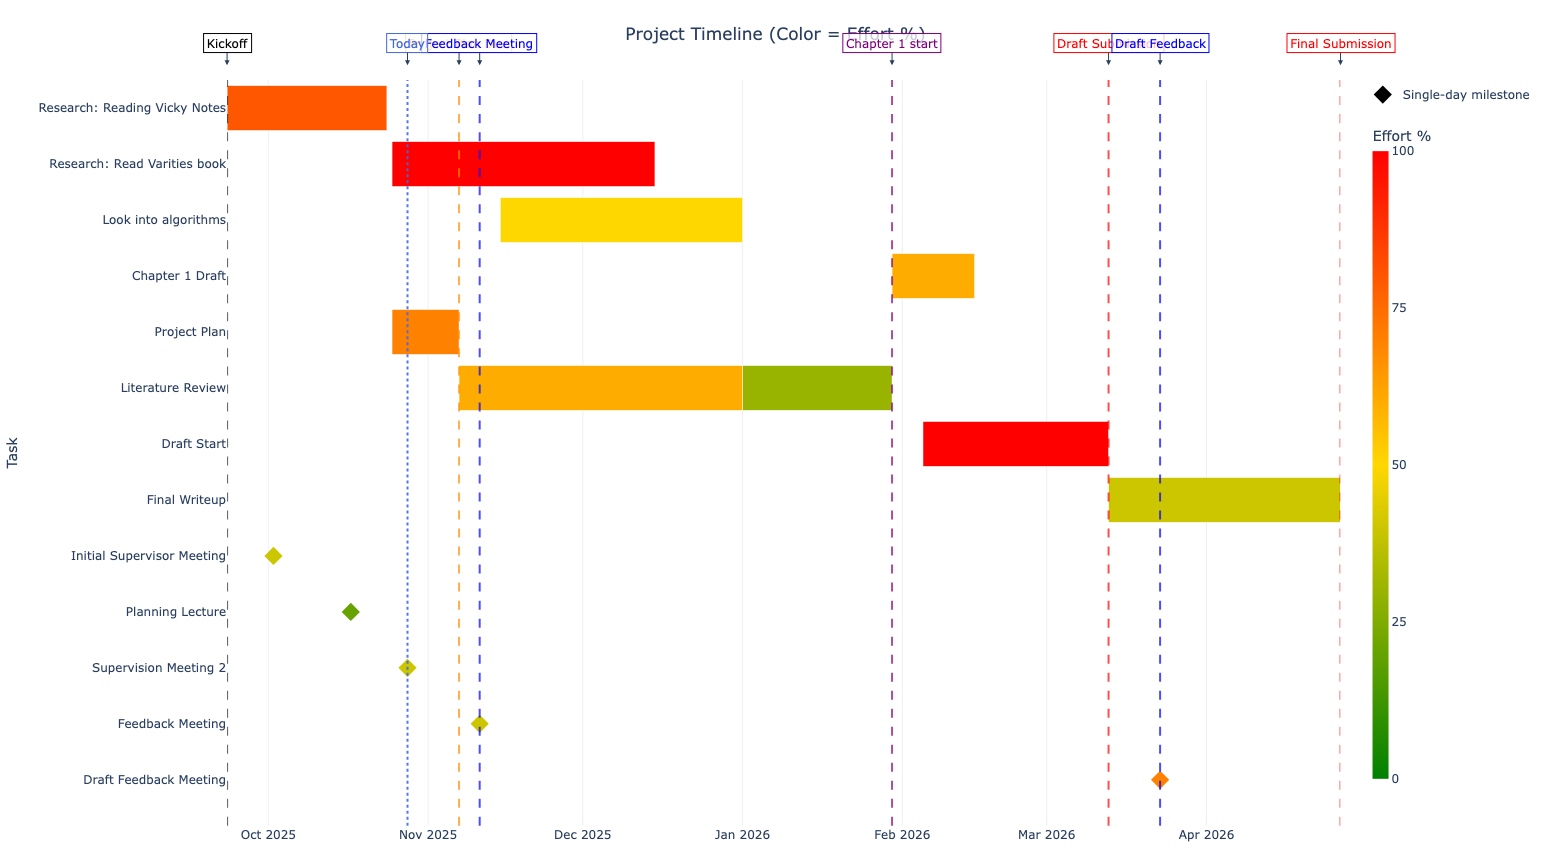
\includegraphics[width=1.2\textwidth]{newplot(3)} % image file name without extension
    \caption{Gantt chart showing the timeline for the MMath independent project.}
    \label{fig:gantt_chart}
\end{figure}

% Make a box with a URL link to interactive Gantt chart
\begin{center}
	\fbox{\parbox{0.9\textwidth}{
		For an interactive version of this Gantt chart, please visit: \\
		\centering
		\url{https://www-users.york.ac.uk/~ag1884/}
	}}
\end{center}

\section*{Written Commentary of plan}
The Gantt chart in Figure~\ref{fig:gantt_chart} outlines the timeline for my MMath independent project. The project is structured into several key phases, each with specific tasks and milestones.

\begin{itemize}
	\item \textbf{Initial Research (Weeks 1-5):}  During this part, I focused on reading the lecure notes of my supervisor Prof Victoria Gould and relevant material from book "Automata and Languages" by John M. Howie. This helped me understand the basics of DFA's and syntactic monoids
	\item \textbf{Project Plan (Weeks 5-6)}: I started working on my project plan. This also relied on me consulting additonal literaturein tandem.
	\item \textbf{Study on Varieties (Weeks 6-12):} This phase involves a deep dive into the theoretical and computational aspects of pseudovarieties of finite monoids and their applications in formal languages and automata theory. I will study Eilenberg's correspondence and related concepts. Most of this material is covered in the book "Varieties of Formal Languages" by Jean-Éric Pin and his lecture notes available online.
	\begin{itemize}
		\item October 25-December 15: Read through relevant chapters of Jean-Éric Pin's book and understand the theoretical concepts.
		\item November 15-January 1: Look into algorithms used to generate syntactic monoids of regular languages and test membership in pseudovarieties.
	\end{itemize}
	
\end{itemize}